\documentclass[sigconf,9pt,nonacm]{acmart}
\settopmatter{printfolios=true}
\renewcommand\footnotetextcopyrightpermission[1]{}
\setcopyright{none}
\pagestyle{plain}
\usepackage{booktabs,array}
\usepackage{xcolor}
\usepackage{xspace}
\usepackage{tikz}
\usetikzlibrary{arrows.meta}
% generated by make_assets_short.py - do not edit
\newcommand{\NCfg}{13}
\newcommand{\NExact}{12}
\newcommand{\NTcp}{14{,}200}
\newcommand{\NStageA}{5{,}200}
\newcommand{\NineShare}{35}
\newcommand{\NModelDiff}{25}
\newcommand{\NStageB}{9{,}000}
\newcommand{\CMaeZero}{0.30}
\newcommand{\CMaxZero}{0.7}
\newcommand{\CWrongZero}{0}
\newcommand{\CMaeOne}{7.39}
\newcommand{\CMaxOne}{99.4}
\newcommand{\CWrongOne}{2}
\newcommand{\CMaeTwo}{14.45}
\newcommand{\CMaxTwo}{99.4}
\newcommand{\CWrongTwo}{4}
\newcommand{\CMaeThree}{21.50}
\newcommand{\CMaxThree}{99.4}
\newcommand{\CWrongThree}{6}
\newcommand{\CN}{28}
\newcommand{\DN}{80}
\newcommand{\DDiff}{10}
\newcommand{\DJoinedWrongDiff}{10}
\newcommand{\DEarlyWrongDiff}{0}
\newcommand{\DJoinedMae}{17.8}
\newcommand{\DEarlyMae}{5.5}
\newcommand{\DJoinedWrong}{14}
\newcommand{\DEarlyWrong}{4}
\newcommand{\DBothWrong}{4}
\newcommand{\EFitEcdsa}{10}
\newcommand{\EFitMlFourFour}{12}
\newcommand{\EFitMlSixFive}{15}
\newcommand{\ECtlN}{36}
\newcommand{\ECtlMax}{0.9}
\newcommand{\ECtlWrong}{0}
\newcommand{\EN}{72}
\newcommand{\RJoinedMae}{1.42}
\newcommand{\RJoinedMax}{98.8}
\newcommand{\RJoinedWrong}{2}
\newcommand{\RJoinedRest}{142}
\newcommand{\RN}{144}
\newcommand{\RJoinedRestMax}{0.85}
\newcommand{\REarlyMae}{0.54}
\newcommand{\REarlyMax}{0.8}
\newcommand{\REarlyWrong}{0}
\newcommand{\REarlyRest}{144}
\newcommand{\RaceN}{221}
\newcommand{\RaceMlN}{134}
\newcommand{\RaceThr}{0.049}
\newcommand{\RaceRight}{132}
\newcommand{\RaceBeforePct}{90}
\newcommand{\RaceTwoRight}{36}
\newcommand{\RaceTwoScored}{36}
\newcommand{\RaceTwoOosRight}{394}
\newcommand{\RaceTwoOosN}{399}
\newcommand{\MixFitExc}{13}
\newcommand{\MixPredExc}{15}
\newcommand{\MixN}{4}
\newcommand{\MixRight}{3}
\newcommand{\NineDefMaeBefore}{13.3}
\newcommand{\NineDefMaeAfter}{1.2}
\newcommand{\NineN}{48}
\newcommand{\NineRwndDefOk}{7}
\newcommand{\NineRwndDefTot}{20}
\newcommand{\NineRwndLargeOk}{16}
\newcommand{\NineRwndLargeTot}{20}
\newcommand{\GenCells}{240}
\newcommand{\GenRespMax}{16}
\newcommand{\GenRttLo}{5}
\newcommand{\GenRttHi}{100}
\newcommand{\GenRateLo}{10}
\newcommand{\GenRateHi}{100}
\newcommand{\GenMtuLo}{1\,280}
\newcommand{\GenMtuHi}{9\,000}
\newcommand{\GenWEcRttFive}{10}
\newcommand{\GenWMFourFourRttFive}{10}
\newcommand{\GenWMSixFiveRttFive}{10}
\newcommand{\GenWEcRttThirty}{10}
\newcommand{\GenWMFourFourRttThirty}{12}
\newcommand{\GenWMSixFiveRttThirty}{15}
\newcommand{\GenWEcSlowTen}{10}
\newcommand{\GenWMFourFourSlowTen}{10}
\newcommand{\GenWMSixFiveSlowTen}{10}
\newcommand{\GenWEcMtuLow}{10}
\newcommand{\GenWMFourFourMtuLow}{12}
\newcommand{\GenWMSixFiveMtuLow}{16}
\newcommand{\ServCells}{48}
\newcommand{\ServWindow}{10}
\newcommand{\ServWrong}{0}
\newcommand{\BkN}{664}
\newcommand{\BkDef}{235}
\newcommand{\BkAOne}{44}
\newcommand{\BkAPct}{23.0}
\newcommand{\BkBRight}{248}
\newcommand{\BkBPct}{57.8}
\newcommand{\NtkRight}{18}
\newcommand{\NtkCells}{18}
\newcommand{\NtkEffect}{7}
\newcommand{\NtkEffectOk}{7}
\newcommand{\HN}{331}
\newcommand{\HLate}{117}
\newcommand{\HEarly}{214}
\newcommand{\HLateSS}{117}
\newcommand{\HWaitMed}{13.7}
\newcommand{\HEarlySS}{19}
\newcommand{\HAOne}{6}
\newcommand{\HALate}{117}
\newcommand{\HAPct}{5.1}
\newcommand{\HEnqMed}{181.2}
\newcommand{\HPcapMed}{-0.073}
\newcommand{\PhAfter}{164}
\newcommand{\PhAfterSS}{164}
\newcommand{\PhBefore}{500}
\newcommand{\PhBeforeSS}{61}
\newcommand{\StN}{799}
\newcommand{\StPOneRight}{799}
\newcommand{\StPOneN}{799}
\newcommand{\StPOnePct}{100.0}
\newcommand{\StPTwoRight}{212}
\newcommand{\StPTwoN}{236}
\newcommand{\StPTwoPct}{89.8}
\newcommand{\StPThreeRight}{51}
\newcommand{\StPThreeN}{74}
\newcommand{\StPThreePct}{68.9}
\newcommand{\StPTwoBRight}{236}
\newcommand{\StPTwoBN}{236}
\newcommand{\StDeferred}{71}
\newcommand{\StDeferredN}{96}
\newcommand{\StLate}{204}
\newcommand{\StLateInflight}{179}
\newcommand{\StLateLimited}{182}
\newcommand{\StEarly}{595}
\newcommand{\StEarlyLimited}{13}
\newcommand{\StBeforeN}{570}
\newcommand{\StBeforePk}{1}
\newcommand{\StAfterN}{204}
\newcommand{\StAfterPk}{10}
\newcommand{\KerN}{288}
\newcommand{\KerBeforeN}{216}
\newcommand{\KerBeforeSS}{0}
\newcommand{\KerAfterN}{72}
\newcommand{\KerAfterSS}{47}
\newcommand{\KerRight}{274}
\newcommand{\KerPct}{95.1}
\newcommand{\KerWrong}{14}
\newcommand{\KerMissLo}{0.039}
\newcommand{\KerMissHi}{0.080}
\newcommand{\KerMissNear}{0.031}
\newcommand{\AblFixedMae}{2.30}
\newcommand{\AblFixedOff}{4}
\newcommand{\AblFixedN}{144}
\newcommand{\AblSlowMae}{1.42}
\newcommand{\AblSlowOff}{2}
\newcommand{\AblSlowN}{144}
\newcommand{\AblLinuxMae}{1.42}
\newcommand{\AblLinuxOff}{2}
\newcommand{\AblLinuxN}{144}
\newcommand{\AblJoinedMae}{1.42}
\newcommand{\AblJoinedOff}{2}
\newcommand{\AblJoinedN}{144}
\newcommand{\AblEarlyMae}{0.54}
\newcommand{\AblEarlyOff}{0}
\newcommand{\AblEarlyN}{144}
\newcommand{\AblCFixedMae}{25.04}
\newcommand{\AblCFixedOff}{7}
\newcommand{\AblCFixedN}{28}
\newcommand{\AblCSlowMae}{35.63}
\newcommand{\AblCSlowOff}{10}
\newcommand{\AblCSlowN}{28}
\newcommand{\AblCLinuxMae}{0.30}
\newcommand{\AblCLinuxOff}{0}
\newcommand{\AblCLinuxN}{28}
\newcommand{\OvTwoSame}{247}
\newcommand{\OvTwoAll}{252}
\newcommand{\OvThreeSame}{247}
\newcommand{\OvThreeAll}{252}
\newcommand{\OvFourSame}{236}
\newcommand{\OvFourAll}{252}
\newcommand{\GxBaseCWrong}{0}
\newcommand{\GxBaseCLoose}{4}
\newcommand{\GxBaseDisEarly}{0}
\newcommand{\GxBaseDisJoined}{10}
\newcommand{\GxBaseEarlyWrong}{4}
\newcommand{\GxBaseMet}{4}
\newcommand{\GxFourCWrong}{0}
\newcommand{\GxFourCLoose}{4}
\newcommand{\GxFourDisEarly}{0}
\newcommand{\GxFourDisJoined}{10}
\newcommand{\GxFourEarlyWrong}{4}
\newcommand{\GxFourMet}{4}
\newcommand{\GxThreeCWrong}{0}
\newcommand{\GxThreeCLoose}{4}
\newcommand{\GxThreeDisEarly}{0}
\newcommand{\GxThreeDisJoined}{10}
\newcommand{\GxThreeEarlyWrong}{4}
\newcommand{\GxThreeMet}{4}
\newcommand{\GxMaxDiff}{0.05}
\newcommand{\CiWinLo}{64.0}
\newcommand{\CiWinHi}{99.8}
\newcommand{\CiJoinedLo}{95.1}
\newcommand{\CiJoinedHi}{99.8}
\newcommand{\CiRaceLo}{94.7}
\newcommand{\CiRaceHi}{99.8}
\newcommand{\CiKerLo}{92.0}
\newcommand{\CiKerHi}{97.3}
\newcommand{\CiNtkEffLo}{59.0}
\newcommand{\CiNtkEffHi}{100.0}
\newcommand{\SignDP}{0.002}
\newcommand{\SignNtkP}{0.016}

\newcommand{\pending}[1]{{\color{red}\textit{[pending: #1]}}}
\newcommand{\ms}{\,ms\xspace}
\newcommand{\citeone}{\cite{paperone}}
\graphicspath{{../Latex/figures/}}
\hyphenation{OpenSSL ac-knowl-edg-ment}
\setlength{\emergencystretch}{2em}

\begin{document}
\title{How Linux Grows the TCP Window After a Short Flight, and What It Costs Post-Quantum TLS in Round Trips}
\author{Trong-Hieu Dinh}
\affiliation{\institution{Banking Academy of Vietnam}\city{Hanoi}\country{Vietnam}}
\email{hieudt@hvnh.edu.vn}
\author{Trong-Minh Hoang}
\authornote{Corresponding author.}
\affiliation{\institution{Posts and Telecommunications Institute of Technology}\city{Hanoi}\country{Vietnam}}
\email{hoangtrongminh@ptit.edu.vn}
\begin{abstract}
Post-quantum signatures stretch TLS flights past the initial TCP window, so the round trips a flight costs depend on the window Linux grew after the previous one. On plain TCP that window obeys a one-line rule, exact in \NExact\ of \NCfg\ configurations: from an initial window of ten, five segments leave ten and six lift it to twelve. Registered predictions refute a larger-window explanation of a model error, and an intervention shows that OpenSSL's separately written session ticket enlarges the server's window. The rule is Reno's and Cubic's; BBR breaks it. The ticket's acknowledgments decide it by arriving before or after the response; why they come late is open, and a timing rule found afterwards is only a machine-dependent proxy. Predictions fixed in advance hold on new cells, under load and on a cable between two machines, but on one random draw five of 100 cells were wrong, all too slow. Five recommendations follow.
\end{abstract}
\begin{CCSXML}
<ccs2012>
<concept><concept_id>10003033.10003039.10003048</concept_id><concept_desc>Networks~Transport protocols</concept_desc><concept_significance>500</concept_significance></concept>
<concept><concept_id>10003033.10003079.10011704</concept_id><concept_desc>Networks~Network measurement</concept_desc><concept_significance>300</concept_significance></concept>
<concept><concept_id>10002978.10003014.10003015</concept_id><concept_desc>Security and privacy~Security protocols</concept_desc><concept_significance>300</concept_significance></concept>
</ccs2012>
\end{CCSXML}
\ccsdesc[500]{Networks~Transport protocols}
\ccsdesc[300]{Networks~Network measurement}
\makeatletter\g@addto@macro\@concepts{\linebreak}\makeatother % break before the second bullet of the CCS concepts
\ccsdesc[300]{Security and privacy~Security protocols}
\keywords{TLS 1.3, post-quantum cryptography, TCP congestion window, measurement, design guidance}
\maketitle

\section{Introduction}
A post-quantum signature is big: 3\,309 bytes for ML-DSA-65, against about 70 for ECDSA-P256, nearly fifty times as many. A certificate chain made of them no longer fits in the 10-segment initial window of Linux~\cite{rfc6928}, and every flight that overflows the window costs a round trip. Dukkipati et al.\ argued for that window from web latency~\cite{dukkipati2010}, and R\"uth et al.\ measured it across the IPv4 address space~\cite{rueth2017}. Both look at the window a connection starts with. We look at what happens next: how far the kernel grows the window after a short flight, which decides whether the following flight (a request carrying a client certificate, say) crosses it. The way the TLS library cuts a flight into writes matters as well.

Measurements of post-quantum handshakes find them slower~\cite{paquin2020,sikeridis2020,sosnowski2023,kampanakis2024}, and the closest studies treat the window as a setting. Henrich et al.\ vary the initial window in an emulated setup with key-exchange algorithms: handshake times rise in steps once the data exceed it, and a larger window removes the extra round trips~\cite{henrich2025}. Chou and Cao see the time to first byte climb in steps as certificate chains cross the initial window, and approximate later windows by doubling; process start-up may mask their resumed times~\cite{chou2026}. Anastasova and Kampanakis put a rise of 51\ms (33\%) at 50\ms RTT down to a client chain larger than the client's initial window (10 segments, against 24 on the server), without resumption~\cite{anastasova2025}. The latest systems study counts the server's TCP segments in full handshakes (five connections per condition) and examines the loss tail; it follows neither the window grown between flights nor resumed connections~\cite{dubetskyy2026}. We found no direct measurement of the window after short flights in this setting.

The rule is trickier than it looks. RFC~5681 describes slow start, and RFC~2861 and its successor RFC~7661 describe window validation~\cite{rfc5681,rfc2861,rfc7661}, and Linux lets the window grow to twice the largest number of packets in flight~\cite{linuxcwnd}. Does a five-segment flight pass the boundary $2\times5=10$? That single inequality decides a round trip. We ran into it through a mistake of our own model. A per-segment transport model, validated against OpenSSL~3.5 transactions~\citeone, was right to within 1\ms\ on \RJoinedRest\ of \RN\ resumed configurations (exact 95\% interval \CiJoinedLo--\CiJoinedHi\%; largest error \RJoinedRestMax\ms) and wrong by a whole round trip on two, both ML-DSA-44 with a large request (99\ms at 100\ms RTT, 29\ms at 30\ms). The cost of a flight cannot be read from its size. So how does Linux grow the window after a short flight, and why did those two transactions pay a round trip less than the model charged?

We make four contributions: (1)~a closed-form window rule for plain TCP (what the kernel's window validation implies), tested in \NCfg\ configurations on \NCombW\ machine-kernel combinations and under packet loss; (2)~the main result, from tests with predictions fixed in advance: OpenSSL's session ticket, a write of its own, grows the server's window through acknowledgments whose effect depends on when the kernel processes them; (3)~repetitions on three OpenSSL releases, on Go's \texttt{crypto/tls} and on GnuTLS, under BBR, with delayed acknowledgments, under background load, on a physical link and on cells drawn at random, with every registered criterion that failed reported as failed; and (4)~five recommendations for budgeting flights.

\section{Method}
The testbed is two network namespaces joined by a virtual link and shaped with \texttt{tc netem}. The main platform is an Intel i7-5600U under Linux 7.0.0-42 with OpenSSL~3.5; Section~\ref{sec:repl} repeats the tests elsewhere. The CPU clock is fixed (performance governor, no turbo). TCP runs over IPv6 without timestamps (MSS = MTU$-60$) and with Reno. Acknowledgments leave at once (\texttt{quickack} routes) unless stated. ``Window'' means the sender's congestion window (\texttt{snd\_cwnd}, in segments), and ``receive window'' the receiver's.

\emph{Plain TCP.} Every measurement opens a fresh connection and writes $n_1$ full segments. A 100-byte reply acknowledges them all, and the window is read from \texttt{TCP\_INFO}. A second flight of $n_2$ segments then goes out, timed, after an 80-byte write that stands in for a TLS Finished. Stage~A reads the window after $n_1=\NOneList$ in \NCfg\ configurations that change one factor at a time: RTT 5--100\ms; 10\,Mbit/s--1\,Gbit/s; MTU 1\,280, 1\,500, 9\,000; initial window 4, 10, 20; delayed ACK; Cubic; timestamps; offload (\NStageA\ connections). Stage~B times second flights in six configurations (\NStageB\ connections).

\emph{TLS with fixed predictions.} The TLS tests use resumed TLS~1.3 with mutual authentication, RTT 100\ms and \NPerCell\ transactions per cell. Four suites (ECDSA-P256, ML-DSA-44, -65, -87) give ClientHellos of \ChSegEc, \ChSegMlFourFour, \ChSegMlSixFive\ and \ChSegMlEightSeven\ segments, because the ClientHello carries the ticket and with it the client certificate. Before each measurement we committed the model's prediction for every cell, under every rule compared. Table~\ref{tab:tests} lists the tests with their outcome: rows 1--5 count the cells wrong by a round trip ($>$50\ms at 100\ms RTT), and none was allowed; rows 6--29 give a share or a count against the registered criteria (thresholds in the supplement), each of which had to be met. The archive lists the commit times of the predictions and of the first results, with checksums (\texttt{PREREGISTRATION\_L1.md}). They are git's own times, not an independent timestamp, and for the kernel and state traces only the analysis scripts with their thresholds preceded the run. Within a cell the interquartile range of the latency has a median of \SpreadMed\ms (at most \SpreadMax\ms) in the ticket-timing and client-window cells, against steps of one RTT.

\section{The Window After a Short Flight}\label{sec:window}
The window after an $n$-segment flight is
\begin{equation}
w(n)=\max\bigl(w_0,\;\min(w_0+n,\;2n)\bigr),
\end{equation}
exactly in \NExact\ of \NCfg\ configurations (exact 95\% interval \CiWinLo--\CiWinHi\%; Fig.~\ref{fig:window}). The configurations change one factor at a time and are not independent samples, so the interval is only descriptive. In words, nothing grows below $n=w_0/2$; between $w_0/2$ and $w_0$ the window is $2n$; beyond $w_0$ every acknowledged segment adds one. The figure plots medians of 20 connections against (1) and its limits $2n$ and $w_0+n$ (dotted).

Three kernel functions produce this (mainline, checked 18 November 2026). With one acknowledgment per segment, \texttt{tcp\_\allowbreak reno\_\allowbreak cong\_\allowbreak avoid} returns at once unless \texttt{tcp\_\allowbreak is\_\allowbreak cwnd\_\allowbreak limited} holds; only then does \texttt{tcp\_\allowbreak slow\_\allowbreak start} add the acknowledged segments. The test holds if the sender was window-limited when it sent (\texttt{is\_\allowbreak cwnd\_\allowbreak limited}, set by \texttt{tcp\_\allowbreak cwnd\_\allowbreak validate} when a flight fills the window) or, in slow start, while $\texttt{snd\_\allowbreak cwnd}<2\,\texttt{max\_\allowbreak packets\_\allowbreak out}$: twice the segments in flight, not twice the window. A flight of $n\ge w_0$ segments fills the window, each of its $n$ acknowledgments adds one, and the window becomes $w_0+n$. A shorter flight leaves the window unfilled with $n$ in flight. The window then grows by one per acknowledgment until it reaches $2n$, and not at all if $w_0\ge 2n$.

A short program that applies this logic reproduces (1) for all \KernPairs\ pairs of $w_0\in\{2,4,10,16,20,32\}$ and $n\le 80$, and the measured window at every point of the window scan except at MTU 9\,000 (\texttt{Simulation/window\_\allowbreak from\_\allowbreak kernel.py}). The rule holds in every configuration of stage A but one, and on every platform of Table~\ref{tab:repl}. At MTU~9\,000, the exception, only \NineShare\% of flights match, and the same logic explains why. The default receive buffer lets the sender have about seven segments of 8\,940 bytes in flight, so the receiver's window stops it before its own does; \texttt{is\_\allowbreak cwnd\_\allowbreak limited} stays false and the window does not grow. With \texttt{tcp\_rmem} raised to 1\,MiB, \NineRwndLargeOk\ of \NineRwndLargeTot\ flight sizes follow (1), against \NineRwndDefOk\ by default. The other \NineFailNW\ (\NineFailLo\ to \NineFailHi\ segments) stay one or two segments below it, and we cannot explain them.

For TLS, the boundary is what counts. With $w_0=10$, $w(5)=\WFive$ and $w(6)=\WSix$: a five-segment ClientHello leaves the window alone, a six-segment one raises it. Our model's own window rule differs from (1) by one segment at odd $n>w_0$, but none of the 238 full-handshake configurations of the companion paper (\PFullA, plus 12 with larger requests) is affected. In stage~B, second flights are predicted with a mean error of \StageBLo--\StageBHi\ms once the model uses the window the kernel really had.

\emph{Loss.} We also dropped 0.1, 0.5 and 1\% of the packets independently in each direction (stage~A, one machine, \GsixConn\ connections; row 19 of Table~\ref{tab:tests}). Wherever no segment is retransmitted, the rule survives: \GsixNoRetxOk\ of \GsixNoRetxN\ such connections (\GsixNoRetxPct\%) end with the window of (1). Loss merely makes a retransmission more likely, in up to \GsixWorstRetx\% of connections at 1\% and 40 segments. We had predicted the share of connections with the window of (1) as $(1-p)^n$, as if any loss broke the rule, and the criterion that at least 24 of the \GsixCells\ cells lie within six points of it failed (\GsixWithin\ did). In the \GsixOff\ cells outside, the rule holds more often than predicted (at 1\% and 40 segments, \GsixWorstMeas\% against \GsixWorstPred\%).

\begin{figure}[t]
\centering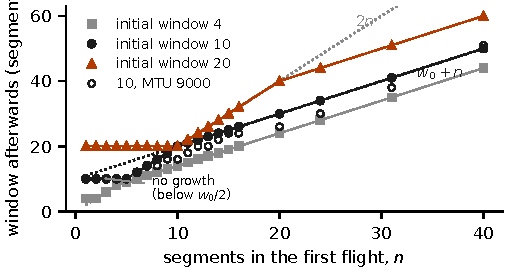
\includegraphics[width=\columnwidth]{fig_window_v3}
\caption{Window after an $n$-segment flight on plain TCP.}
\label{fig:window}
\end{figure}

\section{A Refuted Explanation, and the Ticket}\label{sec:ticket}
\emph{Larger window.} Take ML-DSA-44 with a \CellReq-byte request. The ClientHello is \ChSegMlFourFourW\ segments, so the window stays at 10 and the \CellReqSegsW-segment request flight costs a round trip. The model also put the ticket (about \NstKBMlFourFour\,KB) in the response flight, which then has \CellRespSegsW\ segments and costs a second round trip. The transaction paid only one (\ExMeasMlFourFour\ms against \ExJoinedMlFourFour\ms at 100\ms RTT). A larger window after the ClientHello would explain that. Loosening the rule by two segments, a choice made after seeing the data, takes the round trip off the request flight and brings the mean error down to about \LooseMae\ms over \RN\ configurations. A test with predictions fixed in advance refutes it (Table~\ref{tab:tests}): a 222-byte response, so that only the client's flight can cost a round trip, and request flights of 9--15 segments in \CN\ cells. Fig.~\ref{fig:stagec} shows measured latency as circles, rule~(1) as a solid line and the loosened rule as a dashed one. The step is the extra round trip, and it moves with the size of the ClientHello (\ChSegEc, \ChSegMlFourFour, \ChSegMlSixFive\ and \ChSegMlEightSeven\ segments), which sets the window of the request flight. Rule~(1) is right on all cells (mean error \CMaeZero\ms); the loosened rule is wrong by a round trip on \CWrongTwo. Five models, each adding one element to the one above (a window fixed at $w_0$, textbook slow start, rule~(1), the ticket joined to the response, the ticket written on the Finished), are compared on the \AblFixedN\ resumed configurations and on the \AblCFixedN-cell client-window test (table in the supplement). A window fixed at $w_0$ is wrong on \AblCFixedOff\ of the \AblCFixedN\ client-window cells and textbook slow start on \AblCSlowOff, so the predictions need the validation test.

\begin{figure}[t]
\centering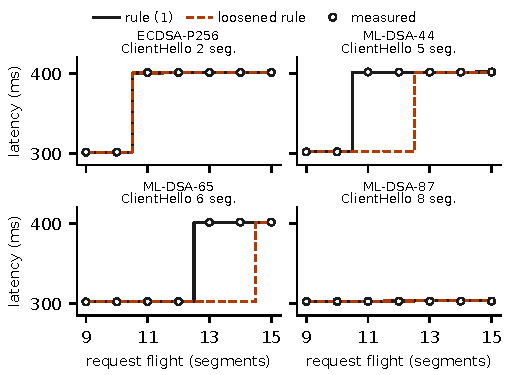
\includegraphics[width=\columnwidth]{fig_stagec_v3}
\caption{Latency of a resumed transaction against the segments of the request flight.}
\label{fig:stagec}
\end{figure}

\emph{Ticket.} The error that remains sits on the server's side. The ticket embeds the client certificate (\NstSegMlFourFour\ to \NstSegMlEightSeven\ segments for ML-DSA-44, -65 and -87), and the model had joined it to the response flight (the joined-ticket model). Suppose OpenSSL writes it separately, the moment the Finished arrives (the early-ticket model, Fig.~\ref{fig:ticket}). When the request flight needs an extra round trip, as for ML-DSA-44, the ticket is acknowledged by the time the response leaves and no longer occupies the window. When it does not, as for ML-DSA-65, ticket and response share the window. Others' data agree: the \DubN\ server segment counts of Dubetskyy and Cano~\cite{dubetskyy2026} come out right only if the two NewSessionTicket messages and the close\_notify alert each leave as a segment of their own (a calculation made after their numbers were published), although those connections did not resume. Removing the ticket fixes ML-DSA-44 but makes ML-DSA-65 a round trip too fast (\CfNoneMlSixFive\ against \CfMeasMlSixFive\ms; post hoc, \texttt{counterfactual\_\allowbreak noticket.py}). The early-ticket model, developed on those \RN\ resumed configurations (so not a test), reproduces them with a mean error of \REarlyMae\ms. A second test with predictions fixed in advance (\DN\ cells; requests of 302 and 19\,460 bytes; responses of 3--12 segments) has \DDiff\ cells where the two models differ by a round trip. The early ticket is right on every one and the joined ticket on none (exact sign test $p=\SignDP$; Table~\ref{tab:tests}).

\emph{The server's window.} Both models fail on the same \DBothWrong\ cells (ML-DSA-44 and -65, a request that needs an extra round trip, responses of 11--12 segments). There the server's window exceeded ten once the ticket was acknowledged, which (1) does not predict. A third test (\EN\ cells, responses of 10--18 segments) maps it. The largest response that avoids an extra round trip is \EFitEcdsa, \EFitMlFourFour\ and \EFitMlSixFive\ segments for tickets of \NstSegEc, \NstSegMlFourFour\ and \NstSegMlSixFive\ segments (ECDSA-P256, ML-DSA-44, -65). With different server and client algorithms the limit follows the client's certificate, hence the ticket, in \MixRight\ of \MixN\ pairs, a small sample (the exception: server ECDSA-P256, client ML-DSA-65, \MixFitExc\ against \MixPredExc). Nor is the window a property of the stack alone. In a \GenCells-cell scan (RTT \GenRttLo--\GenRttHi\ms, \GenRateLo--\GenRateHi\,Mbit/s, MTU \GenMtuLo--\GenMtuHi) the largest response without an extra round trip is \GenWMFourFourRttThirty\ and \GenWMSixFiveRttThirty\ segments for ML-DSA-44 and -65 at 30\ms, and \GenWMFourFourMtuLow\ for ML-DSA-44 at MTU~\GenMtuLo\ (ML-DSA-65 shows no step up to the largest response tested, \GenRespMax\ segments). At \GenRttLo\ms and at \GenRateLo\,Mbit/s, by contrast, every suite stays at \GenWEcRttFive. With server authentication only, where the ticket has one segment, the limit is \ServWindow\ for all three suites, and the early-ticket rule with a window of ten is wrong by a round trip in \ServWrong\ of \ServCells\ cells, as predicted before the measurement.

\emph{What the kernel does with the acknowledgments.} Whether the server's window exceeds ten segments after a ticket does not depend on the order of the ticket's acknowledgment and the response: at least one ticket segment is acknowledged before the response is written in \RaceBeforePct\% of \RaceN\ captured transactions and in \RqKSixPct\% and \RpKSixPct\% of \RpKSixN\ in two repeats with every event on one clock, those where the window stayed at ten included. What separates the outcomes (a finding made afterwards) is the arrival of the ticket's last acknowledgment. When it comes more than \RaceThr\ms after the last request segment, the burst exceeds ten segments in \RaceRight\ of \RaceMlN\ ML-DSA transactions; a request-size sweep with predictions committed beforehand gave the predicted class in \RaceTwoRight\ of \RaceTwoScored\ cells outside a borderline band of \RaceBand\ms. The threshold, fixed on the first run (post hoc), holds in repeats on two x86 machines with the CPU clock fixed (\RpKSevenRight\ to \RqKSevenRight\ of \RoKSevenN, not refitted) but not with the clock left to the system, nor on Arm, with every event on one clock (\RgKSevenRight\ of \RgKSevenN; criterion 90\%), where its agreement with the kernel's state fails too (Section~\ref{sec:repl}), so it is a proxy, not the mechanism, and no constant of Linux TCP. Traces of the server's kernel agree with this reading: \texttt{tcp\_slow\_start} runs exactly when the kernel's own test holds (\StPOneRight\ of \StPOneN\ acknowledgments, as registered). Why the acknowledgments arrive late we could not establish. Both registered explanations failed (socket ownership and the softirq queue, rows 10 and 11 of Table~\ref{tab:tests}). The response burst also equals the window left by the ticket in only \StPTwoPct\% of the transactions (criterion 90\%). A second round read the kernel's counters at every acknowledgment while the client's were delayed by a known amount: on two machines the server's window follows the slow-start rule in \RbEvOk\ of \RbEvN\ acknowledgments, and the burst is the smaller of that window and the response in \RbTxOk\ of \RbTxN\ transactions (the first round failed its registered criteria; the delay moved the order on the Arm machine only; supplement). An intervention at least settles the role of the ticket. When the server issues none on resumed connections (predicted beforehand), the burst is at most ten segments in all \NtkCells\ cells, including the \NtkEffect\ in which it exceeds ten with the ticket (exact sign test on those pairs $p=\SignNtkP$; with seven pairs no result can be smaller).

\begin{figure}[t]
\centering
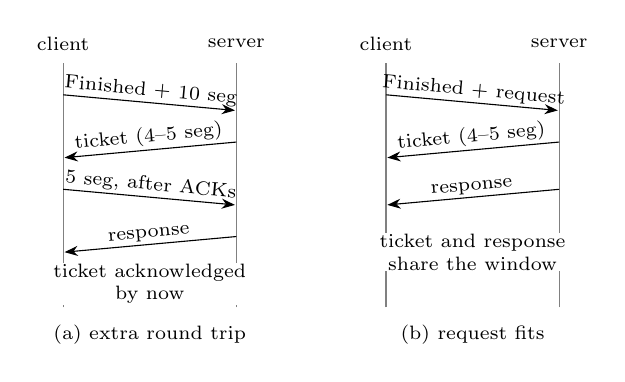
\begin{tikzpicture}[x=1mm,y=1mm,font=\scriptsize,>=Stealth,lab/.style={fill=white,inner sep=0.5pt},a/.style={->,shorten >=0.5pt}]
\foreach \o in {0,41}{\node at (\o,33.5) {client}; \node at (\o+22,33.5) {server}; \draw[gray] (\o,0) -- (\o,31); \draw[gray] (\o+22,0) -- (\o+22,31);}
% (a) the request flight needs an extra round trip
\draw[a] (0,27) -- node[above,sloped,inner sep=1pt] {Finished + 10 seg} (22,25);
\draw[a] (22,21) -- node[above,sloped,inner sep=1pt] {ticket (4--5 seg)} (0,19);
\draw[a] (0,15) -- node[above,sloped,inner sep=1pt] {5 seg, after ACKs} (22,13);
\draw[a] (22,9) -- node[above,sloped,inner sep=1pt] {response} (0,7);
\node[lab,align=center] at (11,3) {ticket acknowledged\\by now};
\node at (11,-3.5) {(a) extra round trip};
% (b) the request fits in the window
\draw[a] (41,27) -- node[above,sloped,inner sep=1pt] {Finished + request} (63,25);
\draw[a] (63,21) -- node[above,sloped,inner sep=1pt] {ticket (4--5 seg)} (41,19);
\draw[a] (63,15) -- node[above,sloped,inner sep=1pt] {response} (41,13);
\node[lab,align=center] at (52,7) {ticket and response\\share the window};
\node at (52,-3.5) {(b) request fits};
\end{tikzpicture}
\caption{Ticket timing: (a) the request flight needs an extra round trip; (b) it does not.}
\label{fig:ticket}
\end{figure}

\begin{table}[t]
\caption{Pre-registered tests and outcomes.}
\label{tab:tests}
\centering\footnotesize\setlength{\tabcolsep}{3pt}
\begin{tabular}{@{}r>{\raggedright\arraybackslash}p{0.57\columnwidth}>{\raggedright\arraybackslash}p{0.31\columnwidth}@{}}
\toprule
 & Test and rule & Result\\
\midrule
1 & Client window: validated rule & \CWrongZero\ of \CN\ (met)\\
2 & Client window: loosened by 2 segments & \CWrongTwo\ of \CN\ (refuted)\\
3 & Ticket joined with response, discriminating cells & \DJoinedWrongDiff\ of \DDiff\ (refuted)\\
4 & Ticket written on Finished, discriminating cells & \DEarlyWrongDiff\ of \DDiff\ (met)\\
5 & Ticket written on Finished, all cells & \DEarlyWrong\ of \DN\\
6 & Request-size sweep, ticket-timing rule, cells outside the borderline band & \RaceTwoRight\ of \RaceTwoScored\ (met)\\
7--11 & Processing of the ticket's acknowledgments (kernel trace, state trace, socket backlog, softirq queue; details in the supplement) & trace \KerRight\ of \KerN; state test \StPOneRight\ of \StPOneN\ (met); burst \StPTwoPct\%, backlog \BkAPct\% and \BkBPct\%, softirq \HAPct\% (not met)\\
12 & No ticket issued: response burst $\le10$ segments & \NtkCells\ of \NtkCells\ (met)\\
13 & Rows 1--5 repeated on OpenSSL 4.1.0 and 3.6.5, same machine, 3.5 as baseline (criteria G1--G4) & \GxFourMet\ (4.1.0) and \GxThreeMet\ (3.6.5) of 4 (met)\\
14 & Rows 1--5 and the ticket position on Go \texttt{crypto/tls} (criteria H1--H5) & \GoMet\ of 5 (not met: H1, H5)\\
15 & Window after a short flight under BBR and under fq pacing, plain TCP (criteria Q1--Q5) & \GelevenMet\ of \GelevenN\ (met)\\
16 & Ticket timing on new cells: RTT 30 and 200\ms, requests of 302--19\,460\,B, OpenSSL~3.5 (criteria K1--K4 per RTT) & \GtwelveMet\ of \GtwelveK\ (met)\\
17 & Client-window and ticket-timing tests under BBR (criteria B1--B5) & \GfBbrMet\ of \GfBbrK\ (met)\\
18 & The same tests with delayed acknowledgments (criteria D1--D5) & \GfDelMet\ of \GfDelK\ (met)\\
19 & Window rule under loss of 0.1, 0.5 and 1\%, plain TCP (criteria L1--L3) & \GsixMet\ of \GsixK\ (not met: L1)\\
20 & Random held-out test: 100 cells drawn from a stated design space (criteria R1--R5) & \GnineMet\ of \GnineK\ (not met: R1, R3, R5)\\
21 & The three BBR cells of row 17 that deviate, measured again with $n=200$ (criteria S1--S2) & \GtwentyMet\ of \GtwentyK\ (met)\\
22 & Tails of six cells, $n=1\,000$ (criteria T1--T2) & \GtwentyoneMet\ of \GtwentyoneK\ (met)\\
23 & Pipelined variant of the model on 60 new Go cells (criteria P1--P4) & \GeighteenMet\ of \GeighteenK\ (met)\\
24 & Background load, four levels: cross traffic, CPU load, both (criteria Y1--Y4) & \GseventeenMet\ of \GseventeenK\ (met)\\
25 & Real link between two machines (criteria F1--F3, and D1--D5 of row 18) & \GthirteenMet\ of \GthirteenK\ (met)\\
26 & The ECDSA-P256 cell of row 20 measured again ($n=200$) and five neighbouring cells that test the ticket size of the model (criteria U1--U4) & \GnineBMet\ of \GnineBK\ (met)\\
27 & Rows 7--11 on one clock, CPU clock fixed: two x86 machines (K1, K2, K4, K5), Arm (D1--D5) & x86 8 of 11 (not met: K1); Arm 3 of 5 (not met: D1, D4)\\
28 & Row 20 on two more machines (criteria A1--A4) & Arm \GnineRepGxMet\ of \GnineRepGxK\ (met), x86 \GnineRepOpMet\ of \GnineRepOpK\ (not met: A2)\\
29 & Rows 16 and 18 on the same machines (criteria K1--K4, D1--D5) & \GtwelveRepMet\ of \GtwelveRepK\ (met)\\
\bottomrule
\end{tabular}
\end{table}

\section{Does It Replicate?}\label{sec:repl}
We repeated the plain-TCP test (stage~A, four configurations, ten repetitions) on four kernels of the i7-5600U (6.8, 6.14, 6.17, 7.0), on an i9-10900K (7.0.0-42, two runs) and on an Arm machine (ASUS Ascent GX10 with an NVIDIA GB10: Cortex-X925 and A725, 6.14 and 7.0). In all \NRunsW\ runs rule~(1) is exact in the base, MTU 1\,280 and $w_0=20$ configurations. At MTU~9\,000 only \MtuLo--\MtuHi\% of the flight sizes match, on every machine alike: the jumbo-frame path (Section~\ref{sec:window}), not a kernel or a CPU. Table~\ref{tab:repl} lists, per platform, the flight sizes with the exact window at MTU~9\,000 and the ticket tests: the state test (\texttt{tcp\_\allowbreak slow\_\allowbreak start} iff the sender is limited), the cells with a burst of at most ten segments without a ticket, and the share of ticket acknowledgments processed from the backlog.

The ticket tests ran on the i7-5600U (7.0) and the Arm machine (6.14 and 7.0), and most results carry over. The state test holds for every acknowledgment. Without a ticket the response burst stays at ten segments or fewer in all \ArmNoTktCells\ cells; the ticket changes \ArmTktChangeW\ of them on Arm, on both kernels, and \NtkEffectW\ on the i7. The two queue explanations fail again: few ticket acknowledgments are processed from the socket backlog on Arm (\BkIPct\% on the i7), and only \ArmLateSixFourteen\ of \ArmLateNSixFourteen\ and \ArmLateSevenZero\ of \ArmLateNSevenZero\ after the write returned (\HALate\ of \HN\ on the i7). Two registered criteria split by machine. The burst criterion is met on Arm (\ArmBurstSixFourteen\% and \ArmBurstSevenZero\%, against \StPTwoPct\% on the i7) and the threshold criterion is not (\ArmThrSixFourteen\% and \ArmThrSevenZero\%, against \StPThreePct\%), so the \RaceThr\ms rule stays a proxy.

\emph{A real link.} Two of the tests were repeated on a cable between two machines (row 25): an i7-8700 client and an i7-5600U server, Linux 7.0.0-42, Intel e1000e NICs at 1\,Gbit/s, offloads on (TSO, GSO, GRO at both ends). The round trip is made with \texttt{tc netem} on both NICs, so the path is real but its delay is not. On plain TCP the median window equals rule~(1) at all \GthirteenSizesN\ sizes at RTT 100 and 30\ms, and \GthirteenConnOk\ of \GthirteenConn\ connections (\GthirteenConnPct\%) end with that window (F1--F3 met). On the cells of row 18 ($n=30$, predictions unchanged) rule~(1) is wrong on \GthirteenCWrong\ of \GthirteenCN\ client-window cells, the early-ticket model on \GthirteenEarlyAll\ of \GthirteenDN\ ticket-timing cells and the joined-ticket model on \GthirteenDiscJoined\ of \GthirteenDisc\ discriminating cells (D1--D5 met).

\begin{table}[t]
\caption{Replication on other kernels and CPUs.}
\label{tab:repl}
\centering\footnotesize\setlength{\tabcolsep}{3pt}
\begin{tabular*}{\columnwidth}{@{\extracolsep{\fill}}lcccc@{}}
\toprule
Platform, kernel & MTU 9\,000 & state & no ticket & backlog\\
\midrule
i7-5600U, 6.8 / 6.14 / 6.17 & \MtuISixEight\ / \MtuISixFourteen\ / \MtuISixSeventeen\% & -- & -- & --\\
i7-5600U, 7.0 & \MtuISevenZero\% & \StPOneRight/\StPOneN & \NtkCells/\NtkCells & \BkIPct\%\\
i9-10900K, 7.0 (2 runs) & \MtuNineI\% & -- & -- & --\\
Arm GX10, 6.14 & \MtuArmSixFourteen\% & \ArmStateSixFourteen/\ArmStateSixFourteen & \ArmNoTktOk/\ArmNoTktCells & \ArmBkSixFourteen\%\\
Arm GX10, 7.0 & \MtuArmSevenZero\% & \ArmStateSevenZero/\ArmStateSevenZero & \ArmNoTktOk/\ArmNoTktCells & \ArmBkSevenZero\%\\
\bottomrule
\end{tabular*}
\end{table}

\section{Other Releases, a Second Library, Other Controllers and Further Tests}\label{sec:other}
\emph{OpenSSL releases.} The code that writes the ticket does not change across the releases we measured. The server's transition after the client's Finished, the flush after the ticket is built and the construction of the ticket are textually identical in 3.5.4, 3.5.9 and 3.6.5. In 4.1.0 the order is unchanged too, though it adds DTLS~1.3 acknowledgments and moves the test of whether to send a ticket into the transition. Full handshakes agree with 3.5.4 in \OvTwoSame, \OvThreeSame\ and \OvFourSame\ of \OvTwoAll\ configurations for 3.5.9, 3.6.5 and 4.1.0, and the rest differ by at most one segment. Reading the source is not measuring, so we repeated the \CN\ client-window cells and the \DN\ ticket-timing cells on 3.6.5 and 4.1.0, with 3.5 as a baseline on the same machine (row 13 of Table~\ref{tab:tests}; predictions and criteria fixed before the run). All four criteria were met on both releases, with the counts of 3.5 (rule (1) wrong on \GxFourCWrong\ of the \CN\ client-window cells, the loosened rule on \GxFourCLoose; the early-ticket model wrong on \GxFourDisEarly\ and the joined-ticket model on \GxFourDisJoined\ of the \DDiff\ discriminating cells) and latencies within \GxMaxDiff\ms of those of 3.5.

\emph{A second library.} Go's \texttt{crypto/tls} writes the ticket with the server's first flight and keeps the client's certificates in it, so the sizes and positions of its writes differ from OpenSSL's. With them calibrated on Go's own probe and the model unchanged, we repeated the two tests (row 14 of Table~\ref{tab:tests}, one machine). Of the \GoKW\ registered criteria, \GoMet\ were met: the first-flight ticket model was wrong on \GoDisGoWrong\ of the \GoDisN\ cells where it differs from the joined-ticket model and on \GoWrongAll\ of \GoDN\ in all. Rule~(1) failed on \GoCWrong\ of \GoCN\ client-window cells (at most two allowed), and the byte check until a \GoClose-byte \texttt{close\_notify} was allowed for (supplement).

\emph{A third library.} GnuTLS~3.8.14 sends two tickets after the client's Finished, each with the client's certificates (\GtlsTicketMinKB\ to \GtlsTicketMaxKB\,KB). We measured it on the X250 and the Arm machine, model unchanged. We varied the ticket data from none to four tickets at the same suite, client window and request: on the \GtlsATInflight\ of \GtlsATN\ cells where the explanations differ, the latency followed the model (the tickets share the server's window of ten), not a window grown by rule~(1) on the ticket flight, so the ticket's size alone does not set the window. The model was wrong on \GtlsADWrong\ of 85 cells and \GtlsARWrong\ of 40 random cells (Arm; \GtlsXDWrong\ and \GtlsXRWrong\ on x86), all too slow, \GtlsSharedWrong\ of them on both machines (supplement).

All \GoWrongSuiteN\ wrong cells are ML-DSA-87, and every one is a round trip faster than predicted. A packet capture shows why. The ML-DSA-87 first flight (\GoChMlEightSeven\ segments) exceeds the window of ten, and the client sends its Finished and request after the first ten segments: the tail of the flight is the end of the ticket, which it need not wait for. Our model treats a flight as complete before the next step begins. A variant that stops charging for the tail, formulated after seeing the data, brings the wrong cells from \GoPostBefore\ to \GoPostAfter. The model follows the ticket once its position is measured, but it has a limit where a flight is longer than the window.

Because the variant was formed after the data, we registered its predictions, and those of the original model, for \GeighteenN\ new ML-DSA-87 cells (RTT 30, 50 and 200\ms, requests of 302 to 19\,460\,B, responses of 3 to 12 segments) and \GeighteenCtlN\ ML-DSA-65 controls whose first flight fits the window (row 23). The variant was wrong on \GeighteenWrongPip\ of the \GeighteenN\ cells, by at most \GeighteenMaxErr\ms, and the original model on all \GeighteenWrongGo; on the controls both agree and the variant's largest error is \GeighteenCtlErr\ms. All four criteria were met. The post hoc variant is therefore a measured description of Go, not a fit to the cells it was made from, on this machine and these sizes.

\emph{Other controllers and pacing.} On plain TCP (stage~A, one machine; row 15 of Table~\ref{tab:tests}), with hypotheses read from the kernel source before the run, all \GelevenN\ criteria were met. Under BBR (the in-tree v1) the window after an $n$-segment flight is $w_0+n$ for every $n$, because its update adds the packets acknowledged without asking whether the sender was limited; rule~(1) is therefore wrong for all \GelBbrWrongW\ sizes $n\le\GelBbrMax$. Under fq pacing with Reno or Cubic the window is that of (1) (\GelCubDiffW\ of \GelCubSizes\ sizes differs, by \GelCubDeltaW\ segments, for Cubic at $n=\GelCubAt$), and a flight within the initial quantum takes as long as on the unpaced baseline.

\emph{The ticket tests under BBR and delayed acknowledgments.} Both were repeated with predictions and criteria fixed in advance (rows 17 and 18; one machine, RTT 100\ms). Under BBR the model with window $w_0+n$ was wrong on \GfBbrCWrong\ of \GfBbrCN\ client-window cells, and rule~(1) on all \GfBbrRuleWrong\ where the two differ. In the ticket-timing cells the BBR model was wrong on \GfBbrDWrong\ of \GfBbrDN, and the model of this paper on \GfBbrRenoWrong\ of the \GfBbrDDiff\ cells where they differ. All \GfBbrK\ criteria were met, but narrowly in stage~D. On the other \GfMidNW\ of those cells (ML-DSA-87) the measurement lies between the models, \GfMidAbove\ms above BBR's prediction and \GfMidBelow\ms below Reno's, so neither is favoured; one ECDSA cell is \GfLow\ms below both. With delayed acknowledgments rule~(1) was wrong on \GfDelCWrong\ of \GfDelCN\ cells and the early-ticket model on \GfDelEarlyAll\ of \GfDelDN\ (the joined-ticket model on \GfDelJoinedDiff\ of the \GfDelDDiff\ discriminating cells); all \GfDelK\ criteria were met.

\emph{Ticket timing on new cells.} We found the ticket hypothesis on \DDiff\ discriminating cells at a single RTT (95\% Wilson interval of the success rate [72, 100]\%), so it needed a test elsewhere. We ran it at RTT 30 and 200\ms with requests of 302 to 19\,460\,B (OpenSSL~3.5, one machine, row 16; \GtwelveCells\ cells, \GtwelveDis\ of them discriminating; predictions and criteria fixed before the run). All \GtwelveK\ criteria were met. The early-ticket model was wrong on \GtwelveEarlyDis\ of the discriminating cells and the joined-ticket model on \GtwelveJoinedDis\ (interval [\GtwelveWilsonLo, 100]\%). Over all \GtwelveCells\ cells the early-ticket model was wrong on \GtwelveEarlyAll, the same cell at both RTTs (ML-DSA-65, 19\,460-byte request, response of 14 segments), where it charges a round trip that was not paid.

\emph{Cells nobody chose.} We drew \GnineN\ cells at random from a stated design space (suite; request 302 to 22\,000\,B; response 222 to 20\,000\,B; RTT 20 to 200\ms; rate 10 to 1\,000\,Mbit/s; MTU 1\,280 to 1\,500; row 20 of Table~\ref{tab:tests}) and fixed the predictions of the model of this paper before the run. It was right to within half an RTT on \GnineOtherN\ of them and to within 2\ms on \GnineWithinTwo, with a mean absolute error of \GnineMaeOther\ms over those \GnineOtherN. Yet only \GnineMet\ of the \GnineK\ registered criteria were met. The model was wrong on \GnineWrongW\ cells (at most three allowed), the mean absolute error over all \GnineN\ cells was \GnineMae\ms (at most 2), and on the \GnineDisc\ cells where the two ticket models differ the early-ticket model was wrong on \GnineDiscEarlyW\ (none allowed). All \GnineWrongW\ errors are one round trip too slow, in flights of \GnineRespLo\ to \GnineRespHi\ segments: \GnineLargeWrongW\ of the \GnineLargeN\ cells with a response of 12 segments or more, \GnineMidWrongW\ of \GnineMidN\ with 9 to 11, \GnineSmallWrongW\ of \GnineSmallN\ with fewer (a split made afterwards). Of these, \TktWrongAfterW\ lie where the server's window after the ticket exceeds ten, which the model does not predict (Section~\ref{sec:ticket}). The fifth, the one discriminating cell that the early-ticket model got wrong (an ECDSA-P256 cell with a small request, where the joined-ticket model was right), is a ticket-size error that we found afterwards: the ticket of the model is \TktDiffLo\ to \TktDiffHi\ bytes larger than the one on the wire, which at the MSS of that cell turns one segment into two. With the measured size the model is right on that cell and on five neighbours tested with predictions fixed first (row 26; details in the supplement). Another \GnineOffNW\ cells, all at \GnineOffRate\,Mbit/s, are off by \GnineOffLo\ to \GnineOffHi\ms.

\emph{Background load.} The tests above run one connection on an idle machine. We repeated \GseventeenCells\ cells (rule (1) and the ticket-timing cells of row 18, predictions unchanged, $n=30$) at four levels in one session: no load; cross traffic on the link (UDP at 40 and ten TCP connections at 2\ Mbit/s each; \GseventeenUdp\ and \GseventeenTcp\ Mbit/s were achieved, about 58\% of the 100\ Mbit/s link); a busy loop on every CPU, including those of the two probes; and both (row 24). The model was wrong on \GseventeenWrongMax\ of the \GseventeenCells\ cells at every level, and the joined-ticket model on \GseventeenJoinedMin\ of the \GseventeenDisc\ discriminating cells at every level. The loads moved the excess of a cell by at most \GseventeenShiftMax\ms against no load, far below one round trip.

\emph{Stability and tails.} The three BBR cells of row 17 that deviate (two ML-DSA-87 cells between the two models, one ECDSA cell below both), measured again with $n=200$, reproduced their first medians to within \GtwentyMaxDiff\ms (criterion 5\ms; row 21): the deviations are stable, not noise. BBR paces its sending (row 15: a burst takes up to \GelBbrBurstMax\ms longer), which the model does not include; this is untested. Six key cells measured with $n=\GtwentyoneMinN$ transactions each (row 22) have one narrow peak: P99 lies at most \GtwentyoneMaxP\ms above the median, P99.9 at most \GtwentyoneMaxPt\ms, the maximum at most \GtwentyoneMaxMx\ms, and no transaction exceeds its median by 20\ms (criterion: at most 1\%). The tail hides no second step of one round trip.

\section{Recommendations and Limits}
The five recommendations hold for the tested stack (Linux 7.0, Reno, OpenSSL~3.5; 3.6.5 and 4.1.0 in the ticket tests). The first, second and fifth rest on (1), the window of Reno and Cubic (under BBR it is $w_0+n$, row 15 of Table~\ref{tab:tests}); the third and fourth rest on the ticket tests.
\begin{enumerate}
\item \emph{Budget each direction and each write in segments of the actual MSS.} A flight costs a round trip when it exceeds the window that the previous flight in the same direction left. Compute that window with (1), not with $w_0$, and count tickets and every other separate write.
\item \emph{Treat the size of the ClientHello as a threshold.} With $w_0=10$, five segments leave the window at \WFive\ and six raise it to \WSix, so a few bytes (a ticket, say) can lift the next client flight across the window and save a round trip: a larger ClientHello is not necessarily a costlier one.
\item \emph{After a ticket, budget the response flight at ten segments.} Ticket and response share the window if the request fits; if it needs an extra round trip, the ticket's acknowledgment can enlarge the server's window to \SrvWinLo--\SrvWinHi\ segments. Ten was pessimistic in the \DBothWrong\ cells where it was wrong, and in all our tests with Reno or Cubic the model was never too fast by half a round trip (\OsFast\ of \OsRuns\ cell-runs).
\item \emph{Measure the server's window on the actual path.} After a ticket it is the window after every acknowledgment of the ticket that the kernel processes while the sender is limited, which depends on RTT, rate, MTU and on when the server's acknowledgments are processed; no rule here predicts it from the network.
\item \emph{Repeat the plain-TCP test on each kernel and TLS library before relying on (1).} Before using jumbo frames, check that the receive buffer holds the flight: otherwise the sender is not window-limited and (1) does not apply.
\end{enumerate}

\emph{Limits: scope of the measurements.} The window rule was tested on \NCombW\ machine-kernel combinations (\NRunsW\ runs), the ticket tests of Table~\ref{tab:repl} on two machines (three runs), those of Section~\ref{sec:other} on one (rows 16 and 18 also on two more, rows 28 and 29) and those of row 25 on a pair. The link is emulated (two network namespaces and \texttt{tc netem}); row 25 uses one cable between two machines (delay again by \texttt{tc netem}), not an Internet path. Loss was tested on plain TCP only, RTT variation not at all. Background load was one fixed mix and a busy loop (row 24). Each measurement used one connection; concurrency, CPU and throughput are untested. A random draw of cells (row 20) found \GnineWrongW\ wrong of \GnineN, \TktWrongAfterW\ of them where the server's window after a ticket exceeds ten, so the model is not a predictor there; \DomLargeWrong\ of the \DomWrongTotal\ wrong cell-runs of its four runs, and all the wrong GnuTLS cells, have a request over 13\,KB (supplement); on two more machines (row 28) it was wrong on \GnineCellsWrongGx\ and \GnineCellsWrongOp\ cells, \GnineCellsEvery\ of them on every machine and run, so the cells that fail depend in part on the machine. The transactions use mutual authentication, \NPerCell\ per cell, and Reno or Cubic, which give the same window at these sizes. At MTU~9\,000 the rule holds only when the receive buffer does not limit the sender (Section~\ref{sec:window}), and \NineFailNW\ flight sizes stay below it even then; the full handshakes belong to the companion paper~\cite{paperone}.\par\emph{Limits: the TLS library.} We used three TLS libraries: OpenSSL (three releases that share the code writing the ticket), Go's \texttt{crypto/tls} on one machine and GnuTLS on two. The window rule and the processing of acknowledgments are Linux's; writing the ticket when the Finished arrives and cutting data into 16-KB record writes are OpenSSL's, and GnuTLS differs in the number and size of its tickets. wolfSSL 5.9.4 (source read, not measured) stores no ML-DSA certificate in its ticket (over 2\,048 bytes), so the size and number of tickets depend on the library too.

\section{Conclusion}
A few bytes can decide a round trip. With an initial window of ten, five ClientHello segments leave the window where it was and six lift it by two, because Linux adds a segment per acknowledgment only while the sender is limited. That boundary explains most of what our model had missed, though not all. Those two transactions led us to the session ticket, which OpenSSL writes on its own and whose acknowledgment can enlarge the server's window by several segments.

The rule is Reno's and Cubic's, and the server's window after a ticket is the kernel's rule applied to acknowledgments whose arrival we cannot yet predict. A practitioner can budget flights with (1) and the five recommendations (where the model is wrong it is too slow, never too fast), then measure the response flight on the real path. We explain one component of the latency of post-quantum TLS, the extra round trips, not the cost of deploying it. A researcher is left with a sharper question: why do those acknowledgments reach the server so late?

\emph{Acknowledgments.} This work was supported by the Intelligently Connected Networks LABoratory (PTIT) and the Banking Academy of Vietnam. 
\par During the preparation of this work, the first author used ChatGPT (OpenAI) and Claude (Anthropic) to assist with routine analysis scripting, language editing, and consistency checks. After using these tools, both authors reviewed, validated, and edited the code and content as needed, and take full responsibility for the content of the published article.
\par\emph{Availability.} Scripts, data, the pre-registered predictions (with commit times) and derived tables are on Zenodo: doi:\allowbreak10.5281/\allowbreak zenodo.\allowbreak24355942 (all versions) and doi:\allowbreak10.5281/\allowbreak zenodo.\allowbreak24417627 (version l1-v1.1). Raw traces: doi:\allowbreak10.5281/\allowbreak zenodo.\allowbreak24384873 and doi:\allowbreak10.5281/\allowbreak zenodo.\allowbreak24419058.

\bibliographystyle{ACM-Reference-Format}
\bibliography{refs}
\end{document}
